\documentclass[11pt,a4paper]{article}

\usepackage[utf8]{inputenc}
\usepackage[T1]{fontenc}
\usepackage[brazil]{babel}
\usepackage{lmodern}
\usepackage{geometry}
\geometry{margin=2.2cm}
\usepackage{microtype}
\usepackage{booktabs}
\usepackage{tabularx}
\usepackage{array}
\usepackage{xcolor}
\usepackage{graphicx}
\usepackage{tikz}
\usetikzlibrary{arrows.meta,positioning,fit,backgrounds,shapes.geometric}
\usepackage{hyperref}
\hypersetup{colorlinks=true,linkcolor=blue!50!black,urlcolor=blue!50!black}

\definecolor{azul}{HTML}{174A7E}
\definecolor{azulclaro}{HTML}{EAF3FA}
\definecolor{verde}{HTML}{E9F5EC}
\definecolor{laranja}{HTML}{C96B24}
\definecolor{cinza}{HTML}{F2F4F5}
\setlength{\parindent}{1.25cm}
\setlength{\parskip}{0.25em}

\begin{document}
\hypersetup{pageanchor=false}
\begin{titlepage}
\thispagestyle{empty}
\begin{center}
{\large\bfseries Universidade do Estado do Rio de Janeiro}\\[0.4em]
{\large Instituto Politécnico do Rio de Janeiro}\\[0.4em]
{\large Engenharia de Computação}

\vfill

{\LARGE\bfseries Trabalho Final de Tópicos Especiais em Redes de Computadores}\\[1em]
{\Large Arquitetura, segmentação e roteamento de uma rede corporativa}

\vfill

{\large Professor Orientador: Guilherme Domingues}\\[0.8em]
{\large Ana Clara de Oliveira Lima}\\[0.3em]
{\large João Vitor Esteves da Cunha}\\[0.3em]
{\large Manoel Rodrigues da Silva}\\[0.3em]
{\large João Marcello Rocha}

\vfill

{\large 2026}
\end{center}
\end{titlepage}

\hypersetup{pageanchor=true}
\pagenumbering{roman}
\thispagestyle{plain}
\section*{Resumo}
\addcontentsline{toc}{section}{Resumo}
Este trabalho descreve uma proposta de rede corporativa composta por conexão à Internet, roteador de borda, firewall, switch central, switches de acesso, pontos de acesso sem fio e uma rede de servidores. São apresentados o papel de cada equipamento, a separação lógica em sub-redes e VLANs, o plano de endereçamento e o encaminhamento de tráfego. A topologia é analisada como um projeto lógico, adotando os endereços, as rotas e a organização de APs especificados neste trabalho.

\clearpage
\thispagestyle{plain}
\tableofcontents
\clearpage
\pagenumbering{arabic}

\section{Visão geral da rede}

A topologia representa uma rede em camadas. O tráfego externo chega pela Internet ao roteador de borda (Cisco ISR 8200), passa pelo firewall FortiGate 60F e segue para o switch core Cisco Catalyst 9300. O switch core distribui a conectividade para os switches de acesso e para a rede de servidores. Os switches de acesso conectam os pontos de acesso (APs), que fornecem Wi-Fi a computadores e outros dispositivos.

Essa organização separa funções: a borda encaminha tráfego entre a rede local e a operadora; o firewall aplica políticas de segurança; o core concentra a comutação; e a camada de acesso conecta os usuários. A segmentação por sub-redes/VLANs limita domínios de broadcast e permite definir políticas diferentes para servidores e usuários.

\subsection{Visão simplificada}

O primeiro diagrama resume o caminho principal do tráfego. A partir do core, a rede se divide entre os servidores e os switches de acesso, que conectam os quatro APs e as quatro redes de clientes.

\begin{center}
\resizebox{0.82\textwidth}{!}{%
\begin{tikzpicture}[
  box/.style={draw=azul,rounded corners,fill=azulclaro,align=center,
    minimum height=0.9cm,text width=3.5cm,font=\small},
  endbox/.style={draw=gray!65,rounded corners,fill=cinza,align=center,
    minimum height=0.9cm,text width=3.6cm,font=\small},
  conn/.style={draw=azul!80!black,thick,-{Latex}},
  fiberconn/.style={draw=laranja,very thick,-{Latex}}
]
\node[box,ellipse] (internet) at (0,0) {Internet\\WAN 1 Gb/s};
\node[box] (edge) at (0,-1.35) {Roteador de borda\\Cisco ISR 8200};
\node[box] (firewall) at (0,-2.7) {Firewall\\FortiGate 60F};
\node[box] (core) at (0,-4.05) {Switch Core\\Catalyst 9300};
\node[endbox] (servers) at (-5.2,-5.6) {Servidores / serviços\\VLAN 50: 10.0.50.0/24};
\node[box] (access) at (5.2,-5.6) {2 switches de acesso\\Catalyst 9200L};
\node[box] (aps) at (5.2,-7.05) {4 APs\\10.0.10.1--.4};
\node[endbox] (clients) at (5.2,-8.5) {Clientes Wi-Fi x4\\DHCP};
\draw[conn] (internet) -- (edge);
\draw[conn] (edge) -- (firewall);
\draw[conn] (firewall) -- (core);
\draw[conn] (core) -- (servers);
\draw[fiberconn] (core) -- (access);
\draw[conn] (access) -- (aps);
\draw[conn,dashed] (aps) -- node[right,font=\scriptsize]{Wi-Fi} (clients);
\end{tikzpicture}%
}
\end{center}

O diagrama completo sintetiza os enlaces e segmentos do projeto. As linhas sólidas representam Ethernet, as tracejadas azuis indicam PoE entre switches e APs, as linhas laranjas representam fibra de 10 Gb/s entre core e acesso, e as linhas verdes tracejadas indicam Wi-Fi. O desenho é lógico e não representa o número exato de portas nem enlaces redundantes.

\clearpage
\thispagestyle{plain}
\begin{center}
{\Large\bfseries Diagrama lógico da rede}\par\vspace{0.6em}
\begin{center}
\resizebox{0.98\textwidth}{!}{%
\begin{tikzpicture}[
  dev/.style={draw=azul,rounded corners,fill=azulclaro,align=center,
    minimum height=0.85cm,text width=3.4cm,font=\small},
  smalldev/.style={draw=azul,rounded corners,fill=white,align=center,
    minimum height=0.65cm,text width=2.5cm,font=\scriptsize},
  cloud/.style={draw=azul,ellipse,fill=azulclaro,align=center,
    minimum width=2.6cm,minimum height=0.9cm,font=\small},
  subnet/.style={draw=gray!65,rounded corners,fill=cinza,align=center,
    text width=2.55cm,minimum height=0.85cm,font=\scriptsize},
  link/.style={draw=azul!80!black,thick,-{Latex}},
  poe/.style={draw=azul!80!black,thick,dashed,-{Latex}},
  fiber/.style={draw=laranja,very thick,-{Latex}},
  wireless/.style={draw=green!50!black,dashed,thick,-{Latex}}
]
\node[cloud] (inet) at (0,0) {Internet\\WAN 1 Gb/s};
\node[dev] (router) at (0,-2.4) {Roteador de borda\\Cisco ISR 8200};
\node[dev] (fw) at (0,-4.8) {Firewall\\FortiGate 60F\\\texttt{10.0.1.1/24}};
\node[dev] (core) at (0,-7.2) {Switch core\\Cisco Catalyst 9300-24T};
\node[dev] (serv) at (7.5,-7.2) {Servidores / aplicações\\Serviços internos\\VLAN 50: \texttt{10.0.50.0/24}};
\node[dev] (sw1) at (-4.8,-10.0) {Switch de acesso 1\\Cisco Catalyst 9200L-24P-4G};
\node[dev] (sw2) at (4.8,-10.0) {Switch de acesso 2\\Cisco Catalyst 9200L-24P-4G};
\node[smalldev] (ap1) at (-8.3,-12.8) {AP 1\\\texttt{10.0.10.1/24}};
\node[smalldev] (ap2) at (-2.8,-12.8) {AP 2\\\texttt{10.0.10.2/24}};
\node[smalldev] (ap3) at (2.8,-12.8) {AP 3\\\texttt{10.0.10.3/24}};
\node[smalldev] (ap4) at (8.3,-12.8) {AP 4\\\texttt{10.0.10.4/24}};
\node[subnet] (wifi1) at (-8.3,-15.6) {Wi-Fi 1 / DHCP\\\texttt{192.168.10.0/24}};
\node[subnet] (wifi2) at (-2.8,-15.6) {Wi-Fi 2 / DHCP\\\texttt{192.168.20.0/24}};
\node[subnet] (wifi3) at (2.8,-15.6) {Wi-Fi 3 / DHCP\\\texttt{192.168.30.0/24}};
\node[subnet] (wifi4) at (8.3,-15.6) {Wi-Fi 4 / DHCP\\\texttt{192.168.40.0/24}};

\draw[link] (inet) -- node[right,font=\scriptsize]{Ethernet 1 Gb/s} (router);
\draw[link] (router) -- node[right,font=\scriptsize]{\texttt{10.0.1.0/24}} (fw);
\draw[link] (fw) -- (core);
\draw[link] (core) -- node[above,sloped,font=\scriptsize]{VLAN 50} (serv);
\draw[fiber] (core) -- (sw1);
\draw[fiber] (core) -- (sw2);
\node[font=\scriptsize,fill=white,inner sep=2pt] at (-3.0,-8.6) {Fibra óptica 10 Gb/s};
\node[font=\scriptsize,fill=white,inner sep=2pt] at (3.0,-8.6) {Fibra óptica 10 Gb/s};
\draw[poe] (sw1) -- (ap1);
\draw[poe] (sw1) -- (ap2);
\draw[poe] (sw2) -- (ap3);
\draw[poe] (sw2) -- (ap4);
\draw[wireless] (ap1) -- (wifi1);
\draw[wireless] (ap2) -- (wifi2);
\draw[wireless] (ap3) -- (wifi3);
\draw[wireless] (ap4) -- (wifi4);
\node[font=\scriptsize,align=center] at (0,-17.4) {\textcolor{azul}{\rule{0.7cm}{1.2pt} Ethernet}\quad
  \textcolor{azul}{\rule[0.2ex]{0.7cm}{1pt} PoE}\quad
  \textcolor{laranja}{\rule{0.7cm}{1.5pt} Fibra}\quad
  \textcolor{green!50!black}{\rule[0.2ex]{0.7cm}{1pt} Wi-Fi}};
\end{tikzpicture}%
}
\end{center}
\end{center}
\clearpage

\section{Conexão com a Internet e borda}

\subsection{Link WAN}
O acesso externo é indicado como uma conexão Ethernet de 1 Gb/s entre a operadora e o roteador. A nuvem Internet representa a rede pública, não um equipamento interno. A disponibilidade, o endereço WAN e os parâmetros fornecidos pela operadora não foram especificados no diagrama e devem ser documentados na configuração real.

\subsection{Roteador de borda Cisco ISR 8200}
O roteador de borda termina o enlace WAN e encaminha pacotes entre a operadora e a rede interna. No desenho, sua interface LAN pertence ao segmento \texttt{10.0.1.0/24}, conectado ao firewall. O equipamento também pode executar funções de roteamento, monitoramento e contingência, caso esses recursos estejam previstos.

O endereço exato da interface LAN do roteador não está legível/especificado. Portanto, não se deve assumir que ele seja o endereço de gateway dos clientes: o projeto aponta o firewall como próximo salto padrão.

\subsection{Firewall FortiGate 60F}
O firewall está identificado com o endereço \texttt{10.0.1.1/24}. Ele inspeciona o tráfego que cruza entre a rede interna e a borda e permite aplicar regras como controle de acesso, tradução de endereços (NAT), registro de eventos e políticas entre segmentos. Por ser o ponto de segurança entre a LAN e a Internet, recomenda-se que o tráfego de entrada seja negado por padrão e liberado somente conforme a necessidade.

\section{Camada de núcleo e camada de acesso}

\subsection{Switch core Cisco Catalyst 9300-24T}
O switch core concentra as conexões dos switches de acesso, da rede de servidores e do firewall. As ligações para os switches de acesso são descritas como fibra óptica de 10 Gb/s com transceptores SFP+. O core pode transportar várias VLANs por enlaces trunk; o roteamento entre VLANs, contudo, deve ser atribuído explicitamente ao firewall ou a interfaces de camada 3 no core. O desenho, sozinho, não determina qual dos dois fará essa função.

\subsection{Switches de acesso Cisco Catalyst 9200L-24P-4G}
Os dois switches de acesso conectam os APs e outros dispositivos cabeados. O modelo indicado oferece portas com suporte a PoE, permitindo alimentar APs pelo próprio cabo Ethernet quando a potência e o padrão do equipamento forem compatíveis. As portas de uplink ligam cada switch ao core; a velocidade real desses uplinks depende dos módulos e da configuração instalados.

\subsection{Power over Ethernet (PoE)}
PoE transporta dados e energia no mesmo cabo de par trançado. Isso simplifica a instalação dos pontos de acesso e reduz a necessidade de tomadas próximas. É necessário conferir o orçamento PoE total dos switches, a classe de consumo dos APs e o cabeamento utilizado.

\section{Rede sem fio}

\subsection{Pontos de acesso}
Os quatro APs são distribuídos entre os dois switches de acesso e pertencem à rede de gerenciamento/intermediária \texttt{10.0.10.0/24}. Seus endereços são \texttt{10.0.10.1}, \texttt{10.0.10.2}, \texttt{10.0.10.3} e \texttt{10.0.10.4}. As redes de clientes são separadas dessa rede e recebem endereços por DHCP nos segmentos \texttt{192.168.10.0/24}, \texttt{192.168.20.0/24}, \texttt{192.168.30.0/24} e \texttt{192.168.40.0/24}.

\subsection{Redes de clientes e DHCP}
Cada AP está associado a uma sub-rede de clientes distinta, com endereços distribuídos por DHCP:
\begin{itemize}
  \item Wi-Fi 1: \texttt{192.168.10.0/24}, atendida pelo AP 1;
  \item Wi-Fi 2: \texttt{192.168.20.0/24}, atendida pelo AP 2;
  \item Wi-Fi 3: \texttt{192.168.30.0/24}, atendida pelo AP 3;
  \item Wi-Fi 4: \texttt{192.168.40.0/24}, atendida pelo AP 4.
\end{itemize}
O servidor DHCP deve fornecer a cada cliente um endereço, máscara, gateway padrão e DNS apropriados. Como há quatro redes distintas, será necessário configurar escopos DHCP separados e garantir que as VLANs correspondentes atravessem os uplinks até o equipamento que fará o roteamento. A relação entre SSIDs, VLAN IDs e APs não foi informada e deve ser definida.

\section{Segmentação lógica: sub-redes e VLANs}

Uma sub-rede define um conjunto de endereços IP e sua máscara; uma VLAN separa logicamente o tráfego de camada 2. Para cada sub-rede de usuários deve existir uma VLAN correspondente (ou uma justificativa para outro desenho), com gateway de camada 3 e regras de acesso. Os números das VLANs dos Wi-Fis não aparecem na imagem.

\begin{table}[h]
\centering
\caption{Segmentos identificados na proposta}
\label{tab:subredes}
\begin{tabularx}{\textwidth}{@{}l l X@{}}
\toprule
\textbf{Segmento} & \textbf{Rede indicada} & \textbf{Finalidade / observação} \\
\midrule
Interconexão de borda & \texttt{10.0.1.0/24} & Liga o roteador de borda ao firewall; os endereços das interfaces devem ser confirmados. \\
Intermediária / gerenciamento & \texttt{10.0.10.0/24} & Rede compartilhada pelos switches de acesso e pelos quatro APs (endereços \texttt{10.0.10.1} a \texttt{10.0.10.4}). \\
VLAN 50 -- servidores & \texttt{10.0.50.0/24} & Servidores, aplicações e serviços internos. Recomenda-se limitar o acesso por política. \\
Wi-Fi 1 & \texttt{192.168.10.0/24} & Clientes sem fio associados ao AP 1; DHCP. \\
Wi-Fi 2 & \texttt{192.168.20.0/24} & Clientes sem fio associados ao AP 2; DHCP. \\
Wi-Fi 3 & \texttt{192.168.30.0/24} & Clientes sem fio associados ao AP 3; DHCP. \\
Wi-Fi 4 & \texttt{192.168.40.0/24} & Clientes sem fio associados ao AP 4; DHCP. \\
\bottomrule
\end{tabularx}
\end{table}

\subsection{VLAN 50 -- servidores}
A VLAN 50 reúne servidores, aplicações e serviços internos no segmento \texttt{10.0.50.0/24}. A separação permite proteger os serviços sem misturá-los diretamente às redes de usuários. O acesso deve ser autorizado por serviço e origem (por exemplo, liberar apenas as portas necessárias), em vez de permitir comunicação irrestrita entre todas as redes.

\section{Roteamento e fluxo de tráfego}

O roteamento encaminha pacotes entre redes IP diferentes. A tabela abaixo reorganiza as rotas que aparecem no resumo da topologia. ``Diretamente conectada'' significa que a interface do equipamento que contém a rota está na própria rede; não identifica, por si só, em qual equipamento essa interface está configurada.

\begin{table}[h]
\centering
\caption{Rotas apresentadas no diagrama}
\label{tab:rotas}
\begin{tabularx}{\textwidth}{@{}l l X@{}}
\toprule
\textbf{Destino} & \textbf{Próximo salto / interface} & \textbf{Interpretação} \\
\midrule
\texttt{10.0.1.0/24} & Diretamente conectada & Segmento de interconexão indicado entre roteador e firewall. \\
\texttt{10.0.10.0/24} & Diretamente conectada & Rede intermediária indicada para acesso/APs. \\
\texttt{10.0.50.0/24} & Diretamente conectada & VLAN de servidores; a interface L3/gateway deve ser identificada. \\
\texttt{192.168.10.0/24} & \texttt{10.0.10.1} (via AP 1) & Rede de clientes Wi-Fi 1; AP 1 é o próximo salto definido no plano. \\
\texttt{192.168.20.0/24} & \texttt{10.0.10.2} (via AP 2) & Rede de clientes Wi-Fi 2. \\
\texttt{192.168.30.0/24} & \texttt{10.0.10.3} (via AP 3) & Rede de clientes Wi-Fi 3. \\
\texttt{192.168.40.0/24} & \texttt{10.0.10.4} (via AP 4) & Rede de clientes Wi-Fi 4. \\
\texttt{0.0.0.0/0} & \texttt{10.0.1.1} (via ISR 8200) & Rota padrão apontando para o firewall, conforme o resumo fornecido. \\
\bottomrule
\end{tabularx}
\end{table}

\clearpage
\thispagestyle{plain}
\begin{center}
{\Large\bfseries Diagrama de segmentação e rotas}\par\vspace{0.8em}
\resizebox{0.96\textwidth}{!}{%
\begin{tikzpicture}[
  routebox/.style={draw=azul,rounded corners,fill=azulclaro,align=center,
    text width=3.15cm,minimum height=0.9cm,font=\small},
  directbox/.style={draw=green!45!black,rounded corners,fill=verde,align=center,
    text width=3.25cm,minimum height=0.9cm,font=\scriptsize},
  clientbox/.style={draw=laranja!85!black,rounded corners,fill=orange!10,align=center,
    text width=3.2cm,minimum height=1.0cm,font=\scriptsize},
  callout/.style={draw=laranja!85!black,rounded corners,fill=orange!10,align=center,
    text width=3.15cm,minimum height=0.9cm,font=\scriptsize},
  routearrow/.style={draw=azul!80!black,thick,-{Latex}}
]
\node[routebox,ellipse] (inetR) at (0,0) {Internet};
\node[routebox] (isrR) at (0,-1.7) {Cisco ISR 8200\\Roteador de borda};
\node[routebox] (fwR) at (0,-3.6) {FortiGate 60F\\\texttt{10.0.1.1/24}};
\node[routebox] (coreR) at (0,-5.5) {Cisco Catalyst 9300\\Switch core};

\node[directbox] (edgeNet) at (-5,-7.8) {\texttt{10.0.1.0/24}\\Diretamente conectada};
\node[directbox] (apNet) at (0,-7.8) {\texttt{10.0.10.0/24}\\Rede dos APs: .1 a .4};
\node[directbox] (serverNet) at (5,-7.8) {\texttt{10.0.50.0/24}\\Direta -- VLAN 50 / servidores};
\node[callout] (defaultR) at (-4.5,-2.65) {Rota padrão\\\texttt{0.0.0.0/0}\\via \texttt{10.0.1.1}};

\node[clientbox] (c1) at (-6,-10.8) {Wi-Fi 1\\\texttt{192.168.10.0/24}\\via \texttt{10.0.10.1} (AP 1)};
\node[clientbox] (c2) at (-2,-10.8) {Wi-Fi 2\\\texttt{192.168.20.0/24}\\via \texttt{10.0.10.2} (AP 2)};
\node[clientbox] (c3) at (2,-10.8) {Wi-Fi 3\\\texttt{192.168.30.0/24}\\via \texttt{10.0.10.3} (AP 3)};
\node[clientbox] (c4) at (6,-10.8) {Wi-Fi 4\\\texttt{192.168.40.0/24}\\via \texttt{10.0.10.4} (AP 4)};

\draw[routearrow] (inetR) -- node[right,font=\scriptsize]{WAN 1 Gb/s} (isrR);
\draw[routearrow] (isrR) -- (fwR);
\draw[densely dashed,draw=laranja!85!black] (defaultR.east) -- (-0.25,-2.65);
\draw[routearrow] (fwR) -- (coreR);
\draw[routearrow] (coreR) -- (edgeNet);
\draw[routearrow] (coreR) -- (apNet);
\draw[routearrow] (coreR) -- (serverNet);
\draw[routearrow] (apNet) -- (c1);
\draw[routearrow] (apNet) -- (c2);
\draw[routearrow] (apNet) -- (c3);
\draw[routearrow] (apNet) -- (c4);
\end{tikzpicture}%
}
\end{center}
\clearpage

O fluxo típico de um cliente Wi-Fi para a Internet é: cliente \(\rightarrow\) AP \(\rightarrow\) switch de acesso \(\rightarrow\) core \(\rightarrow\) firewall \(\rightarrow\) roteador de borda \(\rightarrow\) operadora. O AP encaminha o tráfego sem fio para a rede cabeada; a comunicação entre sub-redes depende do gateway de camada 3 e das rotas correspondentes. O retorno percorre o caminho inverso, respeitando as regras do firewall.

\section{Premissas de configuração e validação}

Este documento adota como referência a descrição fornecida: os quatro APs pertencem à rede \texttt{10.0.10.0/24}, com endereços \texttt{10.0.10.1} a \texttt{10.0.10.4}, e cada endereço é o próximo salto da respectiva rede Wi-Fi de clientes. Para converter o diagrama lógico em configuração operacional, ainda é necessário especificar:
\begin{enumerate}
  \item \textbf{Função de roteamento dos APs:} configurar os APs conforme o papel de próximo salto atribuído no plano de rotas e confirmar a entrega DHCP para cada rede de clientes.
  \item \textbf{IDs de VLAN:} os IDs numéricos das quatro redes Wi-Fi não foram fornecidos. Definir os IDs e quais VLANs serão transportadas nos enlaces trunk entre acesso e core.
  \item \textbf{Camada 3 da VLAN 50:} definir o gateway da rede \texttt{10.0.50.0/24} e as políticas de acesso entre servidores e redes de usuários.
  \item \textbf{Rota padrão:} a rota \texttt{0.0.0.0/0} usa \texttt{10.0.1.1} como próximo salto em direção ao FortiGate. Associar essa rota ao equipamento correto e confirmar o encaminhamento até o ISR 8200.
  \item \textbf{Enlaces e alimentação:} verificar módulos SFP+, velocidade negociada dos uplinks de fibra e orçamento PoE dos switches para os quatro APs.
  \item \textbf{Serviços e segurança:} definir escopos DHCP, DNS e regras de firewall necessárias para acesso à Internet e aos serviços internos.
\end{enumerate}

Essas definições complementam as premissas adotadas e permitem implementar a arquitetura com endereçamento, rotas e políticas coerentes.

\section{Simulador 3D interativo}

Como complemento aos diagramas estáticos, foi desenvolvida uma aplicação web interativa que representa a topologia da rede em três dimensões. O simulador organiza os equipamentos por camadas: Internet, roteador de borda, firewall, switch core, switches de acesso, APs e redes de clientes. Também apresenta um painel contextual ao selecionar cada elemento.

A interface permite girar e aproximar o modelo, filtrar a visualização por infraestrutura, VLANs/sub-redes ou rotas e acompanhar uma simulação animada do tráfego entre a rede Wi-Fi 1 e a Internet. A aplicação foi implementada em HTML, CSS e JavaScript com a biblioteca Three.js.

O simulador está publicado no GitHub Pages e pode ser acessado pelo link: \href{https://manoelpiovesan.github.io/terc/}{\textbf{Abrir simulador 3D da rede}}.

\section{Conclusão}

A solução proposta adota uma arquitetura hierárquica com roteador de borda, firewall, núcleo de comutação, camada de acesso e cobertura Wi-Fi distribuída. A separação entre a rede de servidores e as redes de clientes permite organizar o tráfego e aplicar controles de segurança. A validação dos gateways, das VLANs, dos endereços de gerenciamento dos APs e das rotas é essencial para transformar o esquema lógico em uma configuração operacional. Com essas definições, a rede pode oferecer conectividade estruturada, segmentação e controle do acesso à Internet e aos serviços internos.

\clearpage
\section*{Imagem original da topologia}
\addcontentsline{toc}{section}{Imagem original da topologia}
\begin{center}
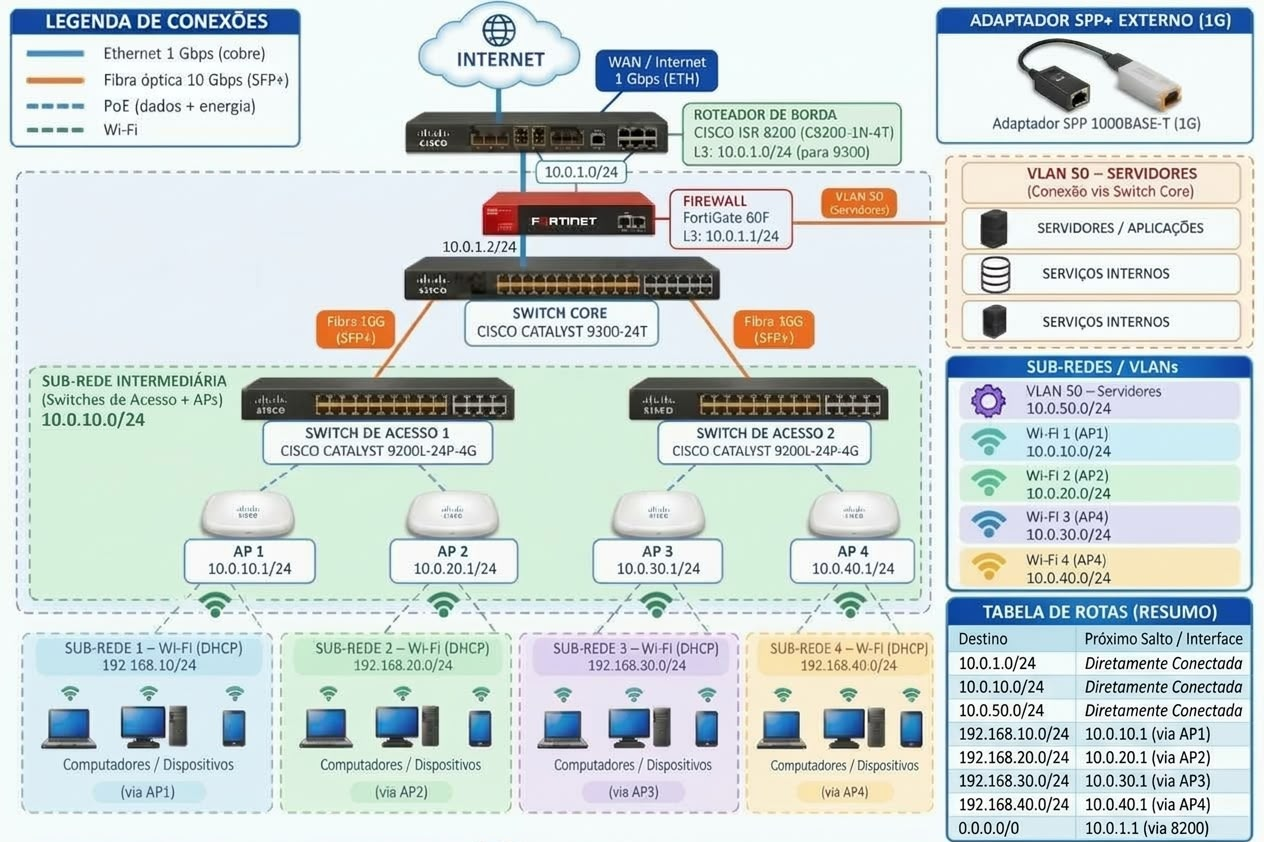
\includegraphics[width=\textwidth,height=0.78\textheight,keepaspectratio]{diagrama_referencia.jpeg}
\end{center}

\end{document}
